\section{Memory}
RAM - Signal\\
ROM - Konstante
\begin{center}
	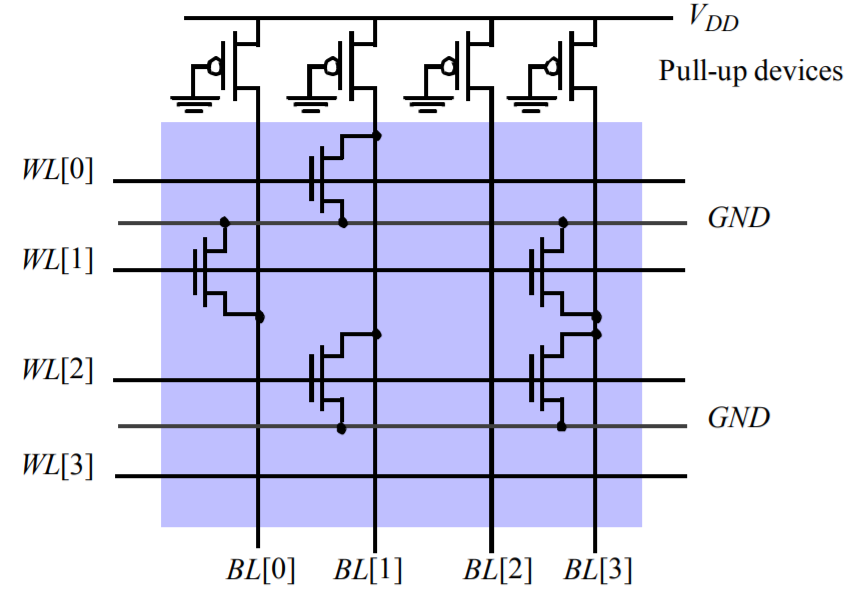
\includegraphics[width=0.5\columnwidth]{Images/rom_matrix.png}
	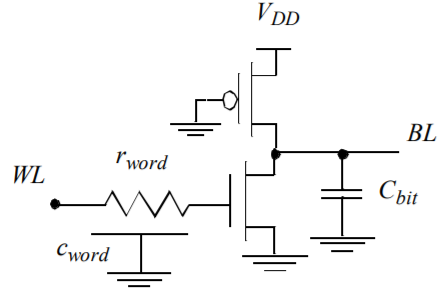
\includegraphics[width=0.45\columnwidth]{Images/basic_cell.png}
\end{center}

\noindent
Die Grösse wird wie folgt vom Speicher beschrieben:
\begin{center}
	\includegraphics[width=0.5\columnwidth]{Images/memory}
\end{center}
Dabei ist Width die Anzahl an Bits pro Wort und Depth die Anzahl möglichen Addressen $Depth=2^{Address\_width}$. 

Die Schnittstelle ist SinglePort RAM, welches ein Zugriff pro Zyklus erlaubt. True DualPort, wobei damit zwei unterschieliche Addressen im gleichen Zyklus gelesen und beschrieben werden können und Simple DualPort, wo ein Port fürs lesen und der andere fürs schreiben zuständig ist.

Geschrieben wird immer synchron. Gelesen kann ein Block synchron und bei verteilten Zugriffen asynchron werden.

\begin{center}
	\includegraphics[width=0.7\columnwidth]{Images/ram_interface}
\end{center}
Beispiel für Single-Port RAM interface:
\begin{lstlisting}
library ieee;
use ieee.std_logic_1164.all;
use ieee.numeric_std.all;

entity RAM is
generic(
  ADDR_WIDTH : integer := 8;
  DATA_WIDTH : integer := 8);
port(
  clk : in std_logic;
  addr:in std_logic_vector(ADDR_WIDTH - 1 downto 0);
  din :in std_logic_vector(DATA_WIDTH - 1 downto 0);
  dout:out std_logic_vector(DATA_WIDTH - 1downto 0);
  we, en: in std_logic ); 
end entity RAM;
\end{lstlisting}

\subsubsection{Operating Modes}
\textbf{Write first}: input data is simultaneously written into memory address location and driven on data output (= transparent).
\textbf{Read first}: data previously stored at address location is driven on data output, while new input data is being stored at address location.
\textbf{No Change Mode}: output latches unchanged during whole write operation. Data at output = previous data.

\subsection{Distributed RAM}
Werte werden in LUTs gespeichert, schreibt synchron und liest asynchron. Dabei können grosse Speicher instaziiert werden, sind aber nur für kleine schnell erreichbar.
\begin{lstlisting}
architecture RTL of RAM is
  constant MEM_DEPTH : integer := 2 ** ADDR_width;
  type ram_type is array (0 to MEM_DEPTH - 1) of std_logic_vector(DATA_width - 1 downto 0);
  signal dist_ram : ram_type;
  
  attribute ram_style : string;
  attribute ram_style of dist_ram: signal is "distributed";
begin -- distributed RAM with asynchronous read
  DistRAM_write : process(clk)
    begin
      if rising_edge(clk) then
        if en = '1' and we = '1' then
	      dist_ram(to_integer(unsigned(addr))) <= din;
	    end if;
	  end if;
	end process DistRAM_write;
	
	AsyncDistRAM_read: dout <= dist_ram(to_integer(unsigned(addr)));
end RTL;
\end{lstlisting}

\subsection{Block RAM}
Werte werden in Block RAMs à 36kb abgespeichert. Schreiben und lesen ist synchron und ist optimiert für Platz und auch schnell für grössere Strukturen.

\begin{lstlisting}
architecture behavioral of RAM is
  constant MEM_DEPTH : integer := 2 ** ADDR_WIDTH;
  type ram_type is array (0 to MEM_DEPTH - 1) of std_logic_vector(DATA_WIDTH - 1 downto 0);
  signal bram : ram_type;

  attribute ram_style : string;
  attribute ram_style of bram: signal is "block";
begin
  sync_BRAM : process(clk)
    begin
      if rising_edge(clk) then
        if en = '1' then -- if RAM is enabled
          if we = '1' then -- if write is enabled
            bram(to_integer(unsigned(addr))) <= din; -- store din in RAM cell
            dout_block <= din; -- read value back
          else -- synchronous read
            dout_block <= bram(to_integer(unsigned(addr)));
          end if;
        end if;
      end if;
    end process sync_BRAM;
end behavioral;
\end{lstlisting}

\subsection{Dual Port RAM}
Shared Variablen halten Werte auch ausserhalb des Prozesses.
\begin{lstlisting}
architecture behavioral of RAM is
  type mem_type is array (0 to (2 **ADDR) - 1) of std_logic_vector(DATA - 1 downto 0);
  shared variable mem : mem_type;
	
begin
  -- Port A
  process(a_clk) 
  begin
    if rising_edge(a_clk) then
      if a_wr = '1' then
        mem(to_integer(unsigned(a_addr))) := a_din;
      end if;
      a_dout <= mem(to_integer(unsigned(a_addr)));
    end if;
  end process;

  -- Port B
  process(b_clk) 
  begin
    if rising_edge(b_clk) then
      if b_wr = '1' then
        mem(to_integer(unsigned(b_addr))) := b_din;
      end if;
      b_dout <= mem(to_integer(unsigned(b_addr)));
    end if;
  end process;
end behavioral;
\end{lstlisting}

\subsection{ROM}
Gleich wie RAM, wobei die gespeicherten Werte keine Signale sondern Konstanten sind.

\subsection{Initialisierung}
Standartmässig werden alle Werte auf 0 gesetzt. Es kann manuell der initiale Zustand bestimmt werden.
\begin{lstlisting}
signal bram: ram_type := ( -- initializes a few ram cells
x"ffff", x"fffe", x"fffd", x"fffc", x"fffb", x"fffa", x"fff9", others => x"0000");
\end{lstlisting}


